In this chapter, the different concepts and definitions regarding Machine Learning, Federated Learning and Blockchain are introduced. These can be regarded as necessary prior knowledge for understanding the remaining chapters of this report.

\section{Machine Learning} \label{preliminaries:machine_learning}

Machine Learning (ML) is a sub-field of Artificial Intelligence that uses algorithms and statistical models in order to detect relevant patterns based on prior experience \cite{geron_2019}. By giving models data, they can learn and adapt without explicit instructions. The data is usually structured as vectors in a multi-dimensional space, such that each vector is an \textit{instance} and each dimension is a \textit{feature}. The remaining of this section will shortly introduce the main categories of Machine Learning.

\subsection{Categories of Machine Learning}

There are three main categories of Machine Learning algorithms: supervised learning, unsupervised learning and reinforcement learning \cite{geron_2019}. Each category performs different tasks in different types of data.

\subsubsection{Supervised Learning}

In supervised learning, algorithms build mathematical models using a set of input samples, which are vectors from a feature space, and expected outputs for each sample. This type of data is known as labeled data, as there is a label for each sample. During a process called training, algorithms provide the model with the input samples and improve the model by comparing its output with the expected outputs. Supervised learning problems can be divided into \textit{regression problems}, if the output is a continuous variable, or \textit{classification problems}, if the output is a discreet variable.

\subsubsection{Unsupervised Learning}

In unsupervised learning, in contrast to supervised learning, algorithms build mathematical models using unlabeled data. Therefore, there are no expected outputs that can be directly compared to the model's output. Some common problems solved by unsupervised learning are \textit{clustering}, \textit{dimensionality reduction} and \textit{anomaly detection}.

\subsubsection{Reinforcement Learning}

In reinforcement learning, models must learn the best action to take according to the current environment, receiving either \textit{rewards} or \textit{penalties} if they perform a good, or bad action, respectively.

\bigskip

This study focuses solely on classification problems in supervised learning settings. Therefore, we always have a labeled data set available.

\section{Federated Learning}

Federated Learning (FL) is a Machine Learning technique where different clients collaboratively train a model under the supervision of an orchestrator. The clients are distributed devices with their own computing resources and data, while the orchestrator is a centralized device that is accessible to all clients. During the training process, the raw data is never exchanged between clients, nor with the central server: only a representation of the model, such as model parameters, is exchanged between devices.

The concept of Federated Learning was introduced by Google researchers in 2016 \cite{10.48550/arxiv.1602.05629}, as an attempt build communication-efficient deep networks in decentralized data settings. Among others, there are different motivations behind building FL systems:

\begin{itemize}
    \item \textit{The central server does not require large computing resources.} The data is produced locally at each client and it is never shared with a central server. In addition, the amount of data at each client is much smaller than the aggregation of all client's data. Since the model is trained at the client's device with their own data, the client's device does not require as many computing resources as a central server would if it trained a model over the aggregation of all client's data.
    
    \item \textit{Models can be trained on sensitive data.} Since the data is produced locally and never shared, a model can be trained over different sensitive data sets without the risk of exposing the sensitive information the data may contain.
    
    \item \textit{There is less data being transported over the network.} During training, only model parameters are required to be shared between devices in order to produce a final model. In addition, model parameters are usually much smaller than the data itself. Therefore, since model parameters are exchanged, there is less data being transported over the network. This can be useful in settings where there is costly or limited network bandwidth.
\end{itemize}

\subsection{Characteristics and Restrictions}

As with any technology, Federated Learning has its own characteristics, restrictions and challenges. Since FL is a novel technology and term, there are various interpretations in the literature of what it actually is. The characteristics and restrictions presented below are based on the survey by Li et al. in 2020 \cite{9084352}.

\begin{itemize}
    \item \textit{Data Locality.} The data is decentralized and distributed across the many clients. Each client is responsible for producing and maintaining their own data, which is never exchanged with other clients, nor the orchestrator. Due to the distributed and decentralized nature of the clients and data, the data is assumed to be non independent or non identically distributed (\textit{non-iid}) across the different clients.
    
    \item \textit{Central Orchestration.} Clients communicate exclusively with the central orchestrator and they never communicate between themselves. The orchestrator takes care of the whole process and never has access to any raw data produced by any client.
    
    \item \textit{System Heterogeneity.} The clients can be heterogeneous in terms of storage, communication and computation capabilities. Therefore, it is imperative that new methods that are developed must take into account that different clients can have different amounts of data, different resources available and take different amounts of processing time.
    
    \item \textit{Privacy Guarantees.} In Federated Learning settings, raw data is never shared between clients and/or with the central orchestrator. However, parameter updates, such as weights, can be target of inference attacks and leak secret information \cite{10.1145/3298981}. Consequently, new innovations must be compatible with techniques that guarantee privacy, such as differential privacy, homomorphic encryption, secure multiparty computation or other cryptographic protocols.
    
    \item \textit{Communication.} Communication is volatile and can be costly. Since clients can be distributed across the globe, the communication latencies can vary. In addition, some clients might be operating in constrained networks with either low or limited bandwidth. Therefore, it is important that FL techniques ensure that communication is minimized.

\end{itemize}

\begin{figure}[!ht]
    \centering
    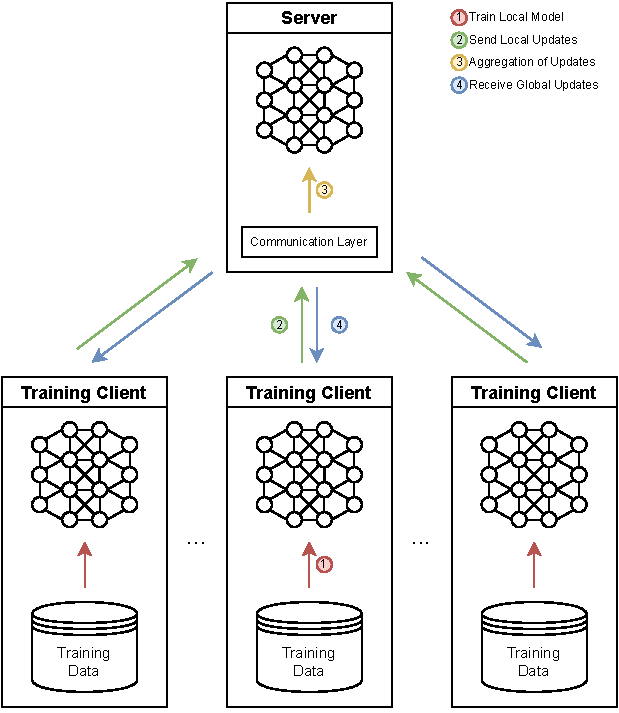
\includegraphics[width=0.8\textwidth]{graphics/hfl-architecture.pdf}
    \caption{Horizontal Federated Learning Architecture}
    \label{fig:hfl_arch}
\end{figure}

\subsection{Categories of Federated Learning}

Federated Learning can be broadly divided into three main categories \cite{10.1145/3298981, 10.1145/3412357} that regard, for the most part, to the different data partition among the clients: Horizontal Federated Learning, Vertical Federated Learning and Federated Transfer Learning.

\subsubsection{Horizontal Federated Learning}

In Horizontal Federated Learning (HFL), clients with the same data structure collaboratively build a single model. In other words, the different data sets in each client share the same feature space, but have a different samples space. For example, two different banks may have very different target user groups (sample space), but their businesses are very similar (feature space). In HFL settings there are usually tens to hundreds of parties and the data is more likely to be equally distributed across the involved parties.

A classic system architecture of HFL is composed by multiple training clients communicating with a central server. As can be seen in \autoref{fig:hfl_arch}, each training client has its own data to train the model. Then, the training client communicates their local updates to the central server. The central server then aggregates the updates and communicates back the global updates. With the global updates, the training clients update their local models to match the global model.

\subsubsection{Vertical Federated Learning}

\begin{figure}[!ht]
    \centering
    \centering
    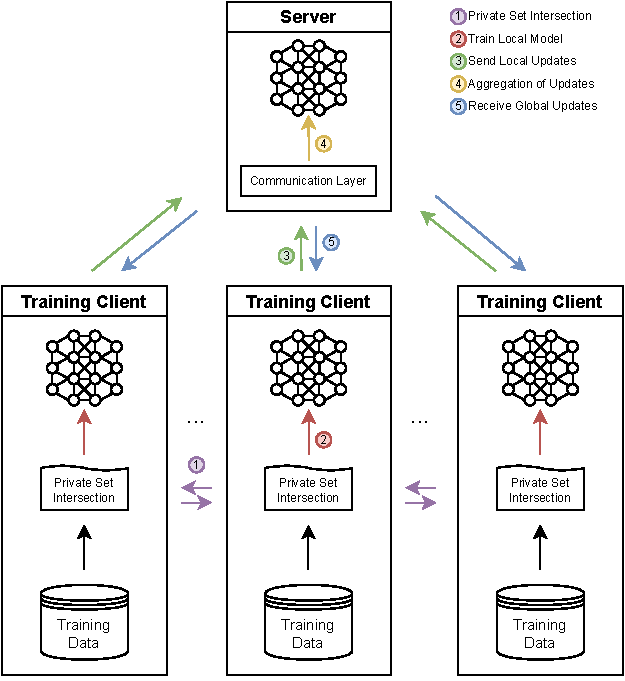
\includegraphics[width=0.8\textwidth]{graphics/vfl-architecture.pdf}
    \caption{Vertical Federated Learning Architecture}
    \label{fig:vfl_arch}
\end{figure}

In Vertical Federated Learning (VFL), clients share an intersecting sample space, but different feature spaces. For example, two companies that operate in the same city have more or less the same client base. However, each company focuses on different areas. In VFL settings, there are usually few parties and the data is more likely to be non-iid.

Similarly to HFL, a classic system architecture of VFL is composed by multiple training clients communicating with a central server. However, there is an important step that needs to be taken into consideration on VFL systems: the Private Set Intersection (PSI). Since not all clients share the exact same sample space, the intersection between all of them has to be calculated before training the model, as can be seen in \autoref{fig:vfl_arch}.

\subsubsection{Federated Transfer Learning}

In Federated Transfer Learning (FTL), clients do not share a sample space, nor a feature space. This technique is similar to regular transfer learning, where a model is previously trained on a data set and then applied to a new similar, but different, data set. For example, two different companies that operate in different countries across the world have a different feature and sample space. However, it may be useful to transfer knowledge between different domains.

\section{Blockchain}
\label{preliminaries:blockchain}

A blockchain is an immutable distributed ledger of transactions maintained by several computers, also known as nodes, linked through a peer-to-peer network. The concept of blockchain was first introduced by Stuart Haber and W. Scott Stornetta in 1991 \cite{10.48550/ARXIV.1810.06130}, being popularized by Satoshi Nakamoto in 2008 with the introduction of the cryptocurrency Bitcoin \cite{nakamoto2009bitcoin}.

\begin{figure}[h]
    \centering
    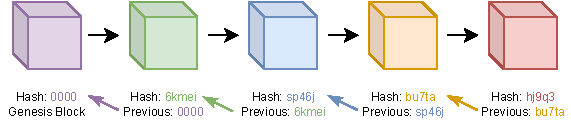
\includegraphics[width=0.8\textwidth]{graphics/blockchain.pdf}
    \caption{Blockchain Representation}
    \label{fig:blockchain_blocks}
\end{figure}

In a blockchain, the data is structured as blocks, as can be seen in \autoref{fig:blockchain_blocks}. Each block contains a certain amount of transactions and links to the previous block via a cryptographic hash, forming a chain. Hence, blockchain. This guarantees fidelity and trust without requiring a trusted third party, which is why it is called a \textit{trustless} system. In addition, since the record is immutable and decentralized, all transactions can be transparently viewed by others.

As mentioned beforehand, a blockchain is maintained by several nodes in a peer-to-peer network. As transactions come in, nodes compete in order to generate the next block. Since it is a decentralized process, multiple nodes will try to create the next block of the chain in parallel. In order to reach an agreement between the nodes, a consensus algorithm is used. The consensus algorithm allows to reach an agreement between multiple decentralized nodes without requiring a singular node to be in charge.

\begin{figure}[h]
    \centering
    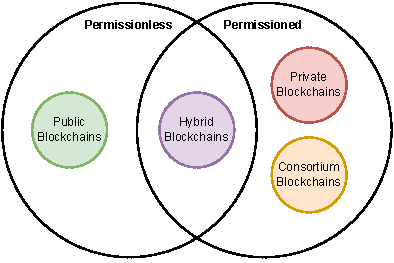
\includegraphics[width=0.5\textwidth]{graphics/blockchain-types.pdf}
    \caption{Blockchain Types}
    \label{fig:blockchain_types}
\end{figure}

There are four different types of blockchain: public, private, consortium and hybrid. Some of these are permissionless, which means that anyone can join the network, while some are permissioned, which means that only allowed parties can join the network. This separation can be visualized in \autoref{fig:blockchain_types}. They work as follows:

\begin{itemize}
    \item \textit{Public Blockchains}. They sit on the permissionless end of the spectrum and therefore anyone can join and participate in the network. There is no central authority.

    \item \textit{Private Blockchains}. In opposition to public blockchains, private blockchains sit on the opposite side of the spectrum, being a permissioned blockchain with a single central authority. This blockchains can only be accessed by allowed parties and they are usually used within organizations.

    \item \textit{Consortium Blockchains}. Similarly to private blockchains, consortium blockchains are also permissioned. However, instead of being controlled by a single authority, they are controlled by a group of different authorities.

    \item \textit{Hybrid Blockchains}. The hybrid blockchains have features of both permisionned and permissionless blockchain systems. On one hand, they are usually controlled by a single authority. On the other hand, they have a mixed usage of permissioned and permissionless protocols running in parallel for different use cases.
\end{itemize}

\subsection{Smart Contracts}

Some blockchain platforms, such as Ethereum \cite{wood2014ethereum}, provide functionality for smart contracts. Smart contracts are small computer programs that live within the blockchain and automatically run when predetermined conditions are met. As they live in the blockchain, they are trustless and are typically used to automate the execution of agreements. This way, every party involved in the agreement is certain that it will be honored once the conditions of the agreement are met.
